\FloatBarrier
\section{The footprint of future interferometric detectors}
\label{sec:adf}
%\input{footprint.tex}

This section briefly reviews the reasoning behind the shape of current gravitational wave detectors and then
discusses alternative geometries which can be of interest for third-generation detectors. We
will use the terminology introduced in the review of a triangular configuration~\cite{Freise09} and
discriminate between the
\emph{geometry}, \emph{topology} and \emph{configuration} of a detector as follows:
\begin{itemize}
\item The \emph{geometry} describes the position information of one or several interferometers,
defined by the number of interferometers, their location and relative orientation.
\item The \emph{topology} describes the optical system formed by its core elements.
The most common examples are the Michelson, Sagnac and Mach--Zehnder topologies.
\item Finally the \emph{configuration} describes the detail of the optical layout and the set of parameters that
can be changed for a given topology, ranging from the specifications of the optical core
elements to the control systems, including the operation point of the main interferometer.\footnote{Note that the
addition of optical components to a given topology is often referred to as a change in configuration.}
\end{itemize}
%%% TODO: the above could do with a bit of a rewrite
\FloatBarrier
\subsection{The L-shape}
Current gravitational wave detectors represent the most precise instruments for measuring length changes.
They are laser interferometers with km-long arms and are operated differently from many precision
instruments built for measuring an absolute length. Viewed from above
they resemble an L-shape with equal arm length.
This geometric form follows directly from the nature of gravitational
waves: gravitational waves are transverse, quadrupole waves, thus a length change measured along any axis
occurs with opposite sign along the axis orthogonal to the previous and the direction of propagation.
This key feature allows to make a differential measurement between two orthogonal interferometer
arms, yielding twice the amplitude of a single arm. More importantly a differential measurement allows us to
potentially discriminate between gravitational wave signals and those types of noise common to both arms, such as,
for example, laser amplitude noise. To achieve this the interferometer arms generally have to have approximately
the same length. The most simple L-shaped interferometer allowing to do this type
of measurement is the symmetric Michelson interferometer, on whose topology all current interferometric detectors
are based.

The long arm length of the detectors represents the simplest way to increase the signal-to-noise ratio
in the detector because the `tidal' effect of the gravitational wave increases with the base length over which the
measurement is taken, while the fundamental noises are connected to the interaction
of light with the optical components or the photo detection and thus do not scale with the length of the interferometer
arms.
%%% adf 31.01.2010 changed the text below because of reviewers 2 comments
We can summarise, provided specifications of the vacuum system housing the interferometer and
the performance of mirror position control systems are good enough, an increase in arm length will increase the
sensitivity of the detector proportionaly.


Using the framework developed in~\cite{Jaranowski98} we can compute the sensitivity of a laser interferometer
with two arms to gravitational waves, taking into account the geometry of the detector, the location of the source and the
changes of both over time. The equations show directly that the arms of the detector do not
have to be perpendicular\footnote{The GEO detector for example features an opening angle of approximately $94^\circ$
in order to make the best use of the available site.}, the right angle, however, provides the maximum
response of an ideal detector to gravitational waves, which more generally can be written as
\begin{equation}
h(t)=F_{+}(t)h_{+}(t)+F_{\times}(t)h_{\times}(t)=\sin\zeta\,f(t,\psi, \dots)
\end{equation}
with $\zeta$ the opening angle of the interferometer arms, $F_{+}$ and $F_{\times}$ the beam pattern functions
and $f(t,\psi, \dots)$ a functions of the remaining parameters describing the geometry (the location of the detector and
of the source in space and time and the wave polarisation angle).

In summary we can say that for a gravitational wave of given direction and polarisation, a properly aligned  symmetric L-shape
is an ideal optical layout for an interferometric
detector; the arms should be as long as possible and the sensitivity is maximised for an opening angle of $90^\circ$.
It should be noted that this does not put severe constraints on the type of interferometer topology used. In fact,
most common interferometer types can be used in a form that features two large symmetric arms in an L-shape
while potential other interferometer arms or sections are shortened such that they can be considered as part of one
corner of the detector.
%%% TODO: maybe add figure? A few example layouts are shown in Figure~\ref{fig:L-layouts} to illustrate this.

\FloatBarrier
\section{Interferometer Topologies }\label{sec:topologies} 
%The typical {\sf L}-shape of current detectors does not necessarily require a Michelson 
%interferometer but can be achieved with other interferometer types, as shown in 
To date no laser interferometer topology other than the Michelson has been
used for gravitational wave detection. However, some very advanced
noise reduction techniques proposed for future 
detectors are based on topologies of the Sagnac interferometer, the Fox-Smith cavity or the
Mach-Zehnder interferometer~\cite{Chen03,danilishin2006,Chen06b}.

It is worth noting that a triangular geometry as discussed above
is conceivable with different interferometer
topologies. In particular it is possible to use different
topologies while maintaining the {\sf L}-shape of the single
interferometers
as displayed in figure~\ref{fig:Lshapes}.
Therefore, for example, three Sagnac interferometers or three cavities
could be used to form a triangle.
Such detector designs can provide similar benefits as described above for the 
triple Michelson geometry so that the triangular geometry is largely independent 
of the topology of the individual interferometers. 
%However, each interferometer topology offers various
%advantages and disadvantages regarding a third generation gravitational wave detector 
%and each should be re-evaluated in this context. 

The case for alternative topologies is largely based on ideas for the
reduction of quantum noise. In general, the signal-to-noise ratio of a 
single interferometer is different for each topology, with the actual
difference depending also on the type of noise under investigation.
However, it is not possible to identify a topology with a meaningful 
signal-to-noise ratio or sensitivity since these vary dramatically
with the interferometer \emph{configuration}. 
%Consequently, detailed
%interferometer designs must be studied for comparing different 
%topologies. To-date such effort has only been fully undertaken for 
%the Michelson topology including ongoing research which shows that the Michelson 
%topology offers interesting possibilities for new 
%quantum noise reduction techniques~\cite{rehbein08}.
\begin{figure}[thb] 
\centering 
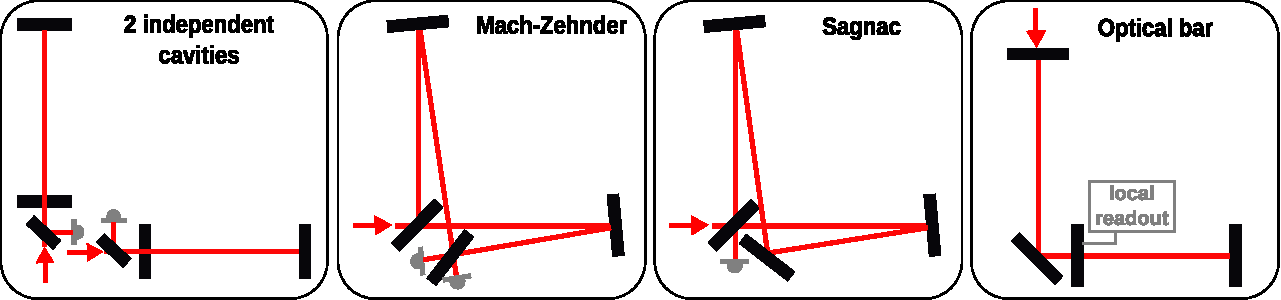
\includegraphics[width=\textwidth]{topologies2}
\caption{Four example interferometer topologies that can be used in a {\sf L}-shaped form: 1) two single cavities
2) Mach-Zehnder interferometer 3) Sagnac interferometer 4) Optical bar.}
\label{fig:Lshapes} 
\end{figure}

During the design and construction of the first generation of detectors 
the Sagnac topology has been investigated and prototypes have been
build~\cite{sun96} but eventually it did not show significant advantages over the Michelson 
topology~\cite{Mizuno97}. More recently it has been proposed to use the Sagnac topology 
as a \emph{speed meter}~\cite{Chen03} to reduce the quantum noise.
The Sagnac topology can be hosted in different ways in a triangular
geometry: each Sagnac as an equilateral triangle, or as an {\sf L}-shaped
zero-area Sagnac. Noise couplings due to the Sagnac effect favor the 
zero-area Sagnac topology: it can be shown that for a typical
choice of optical parameters this extra noise couplings do not
impose stringent new requirements in the case of a zero-area Sagnac
interferometer.

We note that Michelson-based detectors currently offer the 
advantage of using the experience as well as the 
advanced optical technologies of the first two detector generations.


%%% TODO replace png by pdf!!!
\begin{figure}[t]
\begin{center}
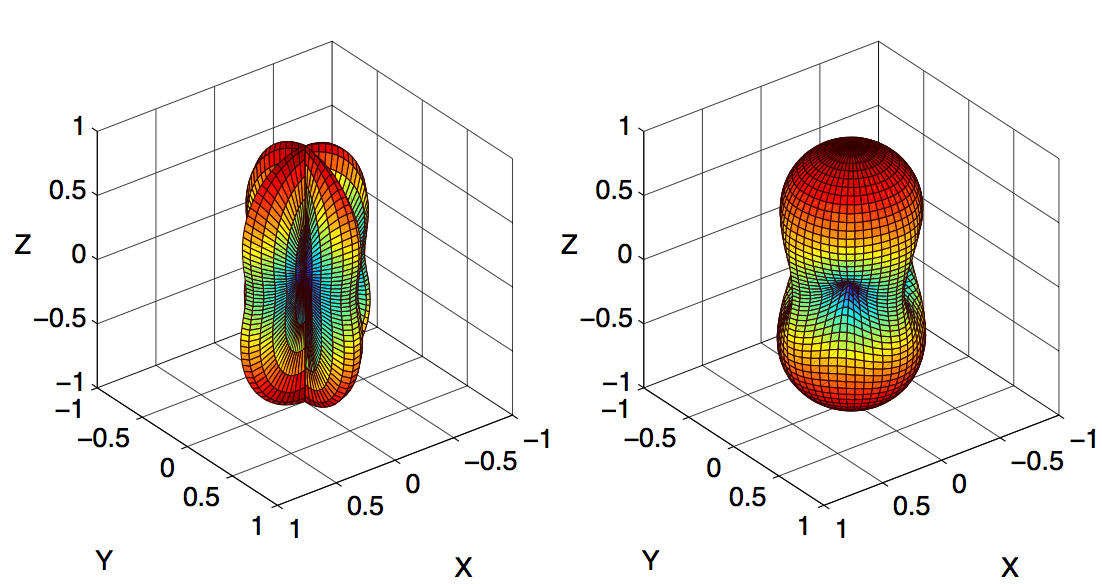
\includegraphics[width=\textwidth]{ap_mi.png}
\caption{
The response of a detector to a linear polarised gravitational wave
as a function of the detector orientation. Both plots show the normalised sensitivity
to a wave travelling along the z-axis. Each data point represents the sensitivity of the
detector for a specific detector orientation defined by the detector normal
passing the respective data point and the origin. The colour
of the data point as well as its distance from the origin indicate the magnitude of the
sensitivity. The left plot depicts the response of a single Michelson, while the right plot
gives the response of a set of three interferometers in a  triangular geometry.
}
\label{fig:triangleAP}
\end{center}
\end{figure}


\FloatBarrier
\subsection{The triangle}
At any given moment an L-shaped detector can only detect one linear combination of polarisations of a
gravitational wave. However, for
estimation of source parameters from the measured signal, the full polarisation information can be essential.
Thus it is of considerable interest to design a detector able to detect both polarisations (and thus the full content)
of a gravitational wave at all times. This can be achieved by combining two co-located
L-shaped detectors which are positioned at $45^\circ$ to each other. % (as shown in Figure~\ref{fig:triangle}).
Already more than 20 years ago it was recognised that a triangular geometry would provide the same
sensitivity to both polarisations as detectors at $45^\circ$ while requiring less enclosed space and fewer
end stations~\cite{Winkler86}. In particular, the sensitivity of the two geometries shown
in Figure~\ref{fig:triangle} differs only by $6\%$~\cite{Freise09}. The difference in the sensitivity to
different polarisations between a single L-shape and a triangular geometry can be best illustrated
with a plot of the so-called antenna pattern as shown in Figure~\ref{fig:triangleAP}.

\begin{figure}[tbh]
\begin{center}
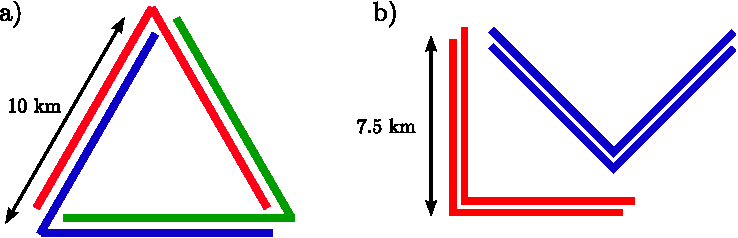
\includegraphics[width=0.7\textwidth,keepaspectratio]{TRIMI03}
\caption{{\bf a)} Triangle geometry: three L-shaped detectors with 10\, km arm length
are positioned in a equilateral triangle.
{\bf b)} Four L-shaped detectors at $0^\circ$ and $45^\circ$. The integrated length of all
interferometer arms in both configurations is 60\,km and two interferometer arms can share
the same structure. Note that for avoiding noise correlations between two detectors the
neighbouring interferometer arms would probably be housed in a separate vacuum tubes.}
\label{fig:triangle}
\end{center}
\end{figure}

Using co-located detectors yields another advantage. Both layouts shown in Figure~\ref{fig:triangle} represent
detectors with redundancy. Redundancy here can be understood in relation to the continuous operation of the
detector as an observatory, or as a feature of the data streams generated by the full system. Redundancy in operation
is achieved by having multiple detectors which generate an equal or similar response to gravitational waves.
This is desirable in observatories which are expected to produce a quasi-continuous stream of astrophysical meaningful
data over an substantial amount of time. Typically laser interferometers cannot produce science data during
upgrades and maintenance work. Thus only alternate upgrading and data taking of redundant detectors can
avoid long down-times, for example during detector upgrades.

Such redundancy is obviously provided in the case of the 4 L-shaped  detectors, where two detectors are
always identical but can be operated independently. However, one can easily show that the triangular geometry
provides exactly the same redundancy~\cite{Freise09}. For example, for three equal L-shaped interferometers
oriented at $0^\circ$, $120^\circ$ and $240^\circ$, one obtains:
\begin{equation}
-h_{0^\circ}= h_{240^\circ}+h_{120^\circ}\,,
\end{equation}
where the sign of the operation is defined by which ports of the interferometers
are used to inject the laser light. Thus the two interferometers at $120^\circ$ and $240^\circ$
create exactly the same response as the one at $0^\circ$. This allows to construct
so-called null-streams (or null-data streams)~\cite{GurselTinto1989}. Null-streams are a powerful
data analysis method that allows to identify noise which is uncorrelated between the
detectors. Even though this does not increase the sensitivity of a detector,
it can add significantly to the robustness of the data processing pipelines and thus lead, for example, to shorter
delays between an event and the generation of a trigger for follow-up searches with optical telescopes.
The triangular geometry represents the minimal setup in one plane that can resolve both polarisations
and provides redundancy for the generation of null-streams.

%The idea of using a triangular geometry is considered with strong interest within the context of
%the design study for a third-generation detector \emph{Einstein gravitational wave Telescope}.
%Therefore we will in the following use the term \emph{ET-class} to refer to three L-shaped detectors in a
%triangular geometry.

